% Options for packages loaded elsewhere
\PassOptionsToPackage{unicode}{hyperref}
\PassOptionsToPackage{hyphens}{url}
\PassOptionsToPackage{dvipsnames,svgnames,x11names}{xcolor}
%
\documentclass[
  letterpaper,
  DIV=11,
  numbers=noendperiod]{scrartcl}

\usepackage{amsmath,amssymb}
\usepackage{iftex}
\ifPDFTeX
  \usepackage[T1]{fontenc}
  \usepackage[utf8]{inputenc}
  \usepackage{textcomp} % provide euro and other symbols
\else % if luatex or xetex
  \usepackage{unicode-math}
  \defaultfontfeatures{Scale=MatchLowercase}
  \defaultfontfeatures[\rmfamily]{Ligatures=TeX,Scale=1}
\fi
\usepackage{lmodern}
\ifPDFTeX\else  
    % xetex/luatex font selection
\fi
% Use upquote if available, for straight quotes in verbatim environments
\IfFileExists{upquote.sty}{\usepackage{upquote}}{}
\IfFileExists{microtype.sty}{% use microtype if available
  \usepackage[]{microtype}
  \UseMicrotypeSet[protrusion]{basicmath} % disable protrusion for tt fonts
}{}
\makeatletter
\@ifundefined{KOMAClassName}{% if non-KOMA class
  \IfFileExists{parskip.sty}{%
    \usepackage{parskip}
  }{% else
    \setlength{\parindent}{0pt}
    \setlength{\parskip}{6pt plus 2pt minus 1pt}}
}{% if KOMA class
  \KOMAoptions{parskip=half}}
\makeatother
\usepackage{xcolor}
\setlength{\emergencystretch}{3em} % prevent overfull lines
\setcounter{secnumdepth}{-\maxdimen} % remove section numbering
% Make \paragraph and \subparagraph free-standing
\makeatletter
\ifx\paragraph\undefined\else
  \let\oldparagraph\paragraph
  \renewcommand{\paragraph}{
    \@ifstar
      \xxxParagraphStar
      \xxxParagraphNoStar
  }
  \newcommand{\xxxParagraphStar}[1]{\oldparagraph*{#1}\mbox{}}
  \newcommand{\xxxParagraphNoStar}[1]{\oldparagraph{#1}\mbox{}}
\fi
\ifx\subparagraph\undefined\else
  \let\oldsubparagraph\subparagraph
  \renewcommand{\subparagraph}{
    \@ifstar
      \xxxSubParagraphStar
      \xxxSubParagraphNoStar
  }
  \newcommand{\xxxSubParagraphStar}[1]{\oldsubparagraph*{#1}\mbox{}}
  \newcommand{\xxxSubParagraphNoStar}[1]{\oldsubparagraph{#1}\mbox{}}
\fi
\makeatother

\usepackage{color}
\usepackage{fancyvrb}
\newcommand{\VerbBar}{|}
\newcommand{\VERB}{\Verb[commandchars=\\\{\}]}
\DefineVerbatimEnvironment{Highlighting}{Verbatim}{commandchars=\\\{\}}
% Add ',fontsize=\small' for more characters per line
\usepackage{framed}
\definecolor{shadecolor}{RGB}{241,243,245}
\newenvironment{Shaded}{\begin{snugshade}}{\end{snugshade}}
\newcommand{\AlertTok}[1]{\textcolor[rgb]{0.68,0.00,0.00}{#1}}
\newcommand{\AnnotationTok}[1]{\textcolor[rgb]{0.37,0.37,0.37}{#1}}
\newcommand{\AttributeTok}[1]{\textcolor[rgb]{0.40,0.45,0.13}{#1}}
\newcommand{\BaseNTok}[1]{\textcolor[rgb]{0.68,0.00,0.00}{#1}}
\newcommand{\BuiltInTok}[1]{\textcolor[rgb]{0.00,0.23,0.31}{#1}}
\newcommand{\CharTok}[1]{\textcolor[rgb]{0.13,0.47,0.30}{#1}}
\newcommand{\CommentTok}[1]{\textcolor[rgb]{0.37,0.37,0.37}{#1}}
\newcommand{\CommentVarTok}[1]{\textcolor[rgb]{0.37,0.37,0.37}{\textit{#1}}}
\newcommand{\ConstantTok}[1]{\textcolor[rgb]{0.56,0.35,0.01}{#1}}
\newcommand{\ControlFlowTok}[1]{\textcolor[rgb]{0.00,0.23,0.31}{\textbf{#1}}}
\newcommand{\DataTypeTok}[1]{\textcolor[rgb]{0.68,0.00,0.00}{#1}}
\newcommand{\DecValTok}[1]{\textcolor[rgb]{0.68,0.00,0.00}{#1}}
\newcommand{\DocumentationTok}[1]{\textcolor[rgb]{0.37,0.37,0.37}{\textit{#1}}}
\newcommand{\ErrorTok}[1]{\textcolor[rgb]{0.68,0.00,0.00}{#1}}
\newcommand{\ExtensionTok}[1]{\textcolor[rgb]{0.00,0.23,0.31}{#1}}
\newcommand{\FloatTok}[1]{\textcolor[rgb]{0.68,0.00,0.00}{#1}}
\newcommand{\FunctionTok}[1]{\textcolor[rgb]{0.28,0.35,0.67}{#1}}
\newcommand{\ImportTok}[1]{\textcolor[rgb]{0.00,0.46,0.62}{#1}}
\newcommand{\InformationTok}[1]{\textcolor[rgb]{0.37,0.37,0.37}{#1}}
\newcommand{\KeywordTok}[1]{\textcolor[rgb]{0.00,0.23,0.31}{\textbf{#1}}}
\newcommand{\NormalTok}[1]{\textcolor[rgb]{0.00,0.23,0.31}{#1}}
\newcommand{\OperatorTok}[1]{\textcolor[rgb]{0.37,0.37,0.37}{#1}}
\newcommand{\OtherTok}[1]{\textcolor[rgb]{0.00,0.23,0.31}{#1}}
\newcommand{\PreprocessorTok}[1]{\textcolor[rgb]{0.68,0.00,0.00}{#1}}
\newcommand{\RegionMarkerTok}[1]{\textcolor[rgb]{0.00,0.23,0.31}{#1}}
\newcommand{\SpecialCharTok}[1]{\textcolor[rgb]{0.37,0.37,0.37}{#1}}
\newcommand{\SpecialStringTok}[1]{\textcolor[rgb]{0.13,0.47,0.30}{#1}}
\newcommand{\StringTok}[1]{\textcolor[rgb]{0.13,0.47,0.30}{#1}}
\newcommand{\VariableTok}[1]{\textcolor[rgb]{0.07,0.07,0.07}{#1}}
\newcommand{\VerbatimStringTok}[1]{\textcolor[rgb]{0.13,0.47,0.30}{#1}}
\newcommand{\WarningTok}[1]{\textcolor[rgb]{0.37,0.37,0.37}{\textit{#1}}}

\providecommand{\tightlist}{%
  \setlength{\itemsep}{0pt}\setlength{\parskip}{0pt}}\usepackage{longtable,booktabs,array}
\usepackage{calc} % for calculating minipage widths
% Correct order of tables after \paragraph or \subparagraph
\usepackage{etoolbox}
\makeatletter
\patchcmd\longtable{\par}{\if@noskipsec\mbox{}\fi\par}{}{}
\makeatother
% Allow footnotes in longtable head/foot
\IfFileExists{footnotehyper.sty}{\usepackage{footnotehyper}}{\usepackage{footnote}}
\makesavenoteenv{longtable}
\usepackage{graphicx}
\makeatletter
\def\maxwidth{\ifdim\Gin@nat@width>\linewidth\linewidth\else\Gin@nat@width\fi}
\def\maxheight{\ifdim\Gin@nat@height>\textheight\textheight\else\Gin@nat@height\fi}
\makeatother
% Scale images if necessary, so that they will not overflow the page
% margins by default, and it is still possible to overwrite the defaults
% using explicit options in \includegraphics[width, height, ...]{}
\setkeys{Gin}{width=\maxwidth,height=\maxheight,keepaspectratio}
% Set default figure placement to htbp
\makeatletter
\def\fps@figure{htbp}
\makeatother

\usepackage{fvextra}
\DefineVerbatimEnvironment{Highlighting}{Verbatim}{breaklines,commandchars=\\\{\}}
 \DefineVerbatimEnvironment{OutputCode}{Verbatim}{breaklines,commandchars=\\\{\}}
\KOMAoption{captions}{tableheading}
\makeatletter
\@ifpackageloaded{tcolorbox}{}{\usepackage[skins,breakable]{tcolorbox}}
\@ifpackageloaded{fontawesome5}{}{\usepackage{fontawesome5}}
\definecolor{quarto-callout-color}{HTML}{909090}
\definecolor{quarto-callout-note-color}{HTML}{0758E5}
\definecolor{quarto-callout-important-color}{HTML}{CC1914}
\definecolor{quarto-callout-warning-color}{HTML}{EB9113}
\definecolor{quarto-callout-tip-color}{HTML}{00A047}
\definecolor{quarto-callout-caution-color}{HTML}{FC5300}
\definecolor{quarto-callout-color-frame}{HTML}{acacac}
\definecolor{quarto-callout-note-color-frame}{HTML}{4582ec}
\definecolor{quarto-callout-important-color-frame}{HTML}{d9534f}
\definecolor{quarto-callout-warning-color-frame}{HTML}{f0ad4e}
\definecolor{quarto-callout-tip-color-frame}{HTML}{02b875}
\definecolor{quarto-callout-caution-color-frame}{HTML}{fd7e14}
\makeatother
\makeatletter
\@ifpackageloaded{caption}{}{\usepackage{caption}}
\AtBeginDocument{%
\ifdefined\contentsname
  \renewcommand*\contentsname{Table of contents}
\else
  \newcommand\contentsname{Table of contents}
\fi
\ifdefined\listfigurename
  \renewcommand*\listfigurename{List of Figures}
\else
  \newcommand\listfigurename{List of Figures}
\fi
\ifdefined\listtablename
  \renewcommand*\listtablename{List of Tables}
\else
  \newcommand\listtablename{List of Tables}
\fi
\ifdefined\figurename
  \renewcommand*\figurename{Figure}
\else
  \newcommand\figurename{Figure}
\fi
\ifdefined\tablename
  \renewcommand*\tablename{Table}
\else
  \newcommand\tablename{Table}
\fi
}
\@ifpackageloaded{float}{}{\usepackage{float}}
\floatstyle{ruled}
\@ifundefined{c@chapter}{\newfloat{codelisting}{h}{lop}}{\newfloat{codelisting}{h}{lop}[chapter]}
\floatname{codelisting}{Listing}
\newcommand*\listoflistings{\listof{codelisting}{List of Listings}}
\makeatother
\makeatletter
\makeatother
\makeatletter
\@ifpackageloaded{caption}{}{\usepackage{caption}}
\@ifpackageloaded{subcaption}{}{\usepackage{subcaption}}
\makeatother

\ifLuaTeX
  \usepackage{selnolig}  % disable illegal ligatures
\fi
\usepackage{bookmark}

\IfFileExists{xurl.sty}{\usepackage{xurl}}{} % add URL line breaks if available
\urlstyle{same} % disable monospaced font for URLs
\hypersetup{
  pdftitle={Lab: K-Means},
  pdfauthor={YOUR NAME HERE},
  colorlinks=true,
  linkcolor={blue},
  filecolor={Maroon},
  citecolor={Blue},
  urlcolor={Blue},
  pdfcreator={LaTeX via pandoc}}


\title{Lab: K-Means}
\author{YOUR NAME HERE}
\date{}

\begin{document}
\maketitle


\begin{tcolorbox}[enhanced jigsaw, opacitybacktitle=0.6, toprule=.15mm, left=2mm, toptitle=1mm, breakable, titlerule=0mm, colframe=quarto-callout-tip-color-frame, arc=.35mm, colback=white, colbacktitle=quarto-callout-tip-color!10!white, opacityback=0, bottomtitle=1mm, coltitle=black, title=\textcolor{quarto-callout-tip-color}{\faLightbulb}\hspace{0.5em}{Getting Started}, leftrule=.75mm, rightrule=.15mm, bottomrule=.15mm]

\begin{enumerate}
\def\labelenumi{\arabic{enumi}.}
\item
  Download the \texttt{.qmd} file from Moodle and any needed
  \texttt{.xlsx} or \texttt{.csv} data files. Save these in the
  \emph{same folder/directory}.
\item
  Open the Quarto file in RStudio:
  \texttt{File\ \textgreater{}\ Open\ File...\ \textgreater{}}. If
  you're working on the MHC RStudio server, you need to upload the files
  first: go to the \texttt{Files} panel, then click \texttt{Upload}.
  Upload the \texttt{.qmd} file and any data files. You will need to
  upload each file one at a time.
\item
  Update the author and date in the YAML header of this file.
\item
  Click the \texttt{Render} button. If successful, you should have a new
  window pop up with a nice looking HTML document.
\item
  For this lab, you \textbf{may need} to still the package
  \texttt{glmnet}.
\end{enumerate}

\textbf{Ask for help} if you encounter issues on any of the steps above.
Once you've successfully made it through these steps, you can continue.

\end{tcolorbox}

\section{Load Packages}\label{load-packages}

You likely will need to install some these packages before you can run
the code chunk below successfully.

\begin{Shaded}
\begin{Highlighting}[]
\FunctionTok{library}\NormalTok{(tidyverse)}
\FunctionTok{library}\NormalTok{(palmerpenguins)}
\FunctionTok{library}\NormalTok{(factoextra)}
\FunctionTok{library}\NormalTok{(amap)}
\end{Highlighting}
\end{Shaded}

\section{Load Penguin Data}\label{load-penguin-data}

\begin{Shaded}
\begin{Highlighting}[]
\FunctionTok{data}\NormalTok{(penguins)}
\end{Highlighting}
\end{Shaded}

\section{Data Cleaning}\label{data-cleaning}

\begin{Shaded}
\begin{Highlighting}[]
\CommentTok{\# Remove missing values}
\CommentTok{\# YOUR CODE HERE}
\NormalTok{penguins }\OtherTok{\textless{}{-}}\NormalTok{ penguins }\SpecialCharTok{\%\textgreater{}\%}
  \FunctionTok{filter}\NormalTok{(}\SpecialCharTok{!}\FunctionTok{is.na}\NormalTok{(bill\_length\_mm) }\SpecialCharTok{\&} \SpecialCharTok{!}\FunctionTok{is.na}\NormalTok{(bill\_depth\_mm) }\SpecialCharTok{\&} \SpecialCharTok{!}\FunctionTok{is.na}\NormalTok{(species))}
\CommentTok{\# Make data table (named penguins\_reduced) that only has}
\CommentTok{\# bill\_length\_mm and bill\_depth\_mm columns}
\NormalTok{penguins\_reduced }\OtherTok{\textless{}{-}}\NormalTok{ penguins }\SpecialCharTok{\%\textgreater{}\%} \FunctionTok{select}\NormalTok{(bill\_length\_mm, bill\_depth\_mm)}
\end{Highlighting}
\end{Shaded}

\section{Initial Visualization}\label{initial-visualization}

\begin{Shaded}
\begin{Highlighting}[]
\FunctionTok{ggplot}\NormalTok{(penguins, }\FunctionTok{aes}\NormalTok{(}\AttributeTok{x =}\NormalTok{ bill\_length\_mm, }\AttributeTok{y =}\NormalTok{ bill\_depth\_mm)) }\SpecialCharTok{+} 
  \FunctionTok{geom\_point}\NormalTok{() }
\end{Highlighting}
\end{Shaded}

\begin{center}
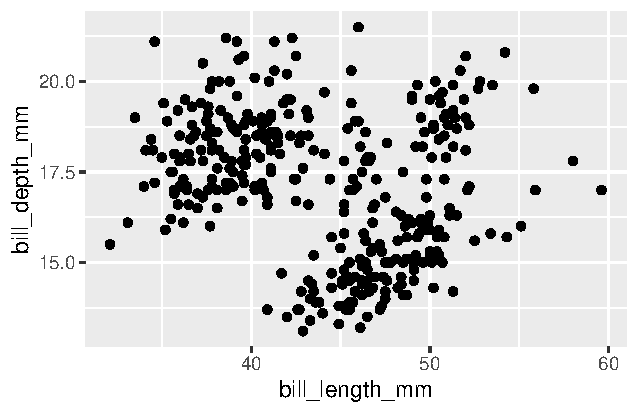
\includegraphics{K-Means-Mini-Demo_files/figure-pdf/unnamed-chunk-5-1.pdf}
\end{center}

We'll cluster these penguins based on their bill lengths and depths:

\section{\texorpdfstring{Implement
\(K\)-Means}{Implement K-Means}}\label{implement-k-means}

Complete the code below to run the K-means algorithm using K = 3.

\begin{Shaded}
\begin{Highlighting}[]
\FunctionTok{set.seed}\NormalTok{(}\DecValTok{244}\NormalTok{)}
\CommentTok{\# Run the K{-}means algorithm}
\NormalTok{kmeans\_3\_round\_1 }\OtherTok{\textless{}{-}} \FunctionTok{kmeans}\NormalTok{(}\FunctionTok{scale}\NormalTok{(penguins\_reduced), }\AttributeTok{centers =} \DecValTok{3}\NormalTok{) }
    
\CommentTok{\# Plot the cluster assignments}
\NormalTok{penguins\_reduced }\SpecialCharTok{\%\textgreater{}\%} 
  \FunctionTok{mutate}\NormalTok{(}\AttributeTok{kmeans\_cluster =} \FunctionTok{as.factor}\NormalTok{(kmeans\_3\_round\_1}\SpecialCharTok{$}\NormalTok{cluster)) }\SpecialCharTok{\%\textgreater{}\%}
  \FunctionTok{ggplot}\NormalTok{(}\FunctionTok{aes}\NormalTok{(}\AttributeTok{x =}\NormalTok{ bill\_length\_mm, }\AttributeTok{y =}\NormalTok{ bill\_depth\_mm, }\AttributeTok{color =}\NormalTok{ kmeans\_cluster)) }\SpecialCharTok{+} 
  \FunctionTok{geom\_point}\NormalTok{(}\AttributeTok{size =} \DecValTok{3}\NormalTok{) }\SpecialCharTok{+} 
  \FunctionTok{theme}\NormalTok{(}\AttributeTok{legend.position =} \StringTok{"none"}\NormalTok{) }\SpecialCharTok{+} 
  \FunctionTok{labs}\NormalTok{(}\AttributeTok{title =} \StringTok{"K{-}means with K = 3 (round 1)"}\NormalTok{) }\SpecialCharTok{+} 
  \FunctionTok{theme\_minimal}\NormalTok{()}
\end{Highlighting}
\end{Shaded}

\begin{center}
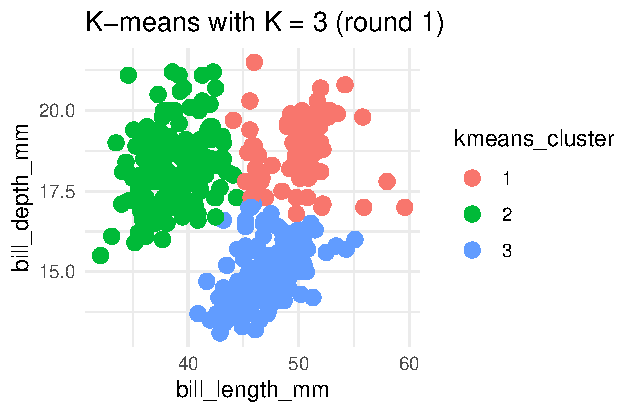
\includegraphics{K-Means-Mini-Demo_files/figure-pdf/unnamed-chunk-6-1.pdf}
\end{center}

\begin{itemize}
\tightlist
\item
  Why do we have to set the seed for K-means? In practice, why should we
  try out a variety of seeds?
\end{itemize}

\textbf{Answer.} For reproducibility every time, we run the function
\(kmeans\), it initializes the centers of the clusters to be in random
location. It's possible that some random location have netter clustering
results than others, since \(kmenas\) is greedy algorithm, it's possible
for it to have different results each time and its possible for it to
get ``stuck''at a local soultion.

\section{K-Means Clusters Versus Known Species
Groupings}\label{k-means-clusters-versus-known-species-groupings}

\begin{Shaded}
\begin{Highlighting}[]
  \FunctionTok{ggplot}\NormalTok{(}\AttributeTok{data =}\NormalTok{ penguins, }\FunctionTok{aes}\NormalTok{(}\AttributeTok{x =}\NormalTok{ bill\_length\_mm, }\AttributeTok{y =}\NormalTok{ bill\_depth\_mm, }\AttributeTok{color =}\NormalTok{ species)) }\SpecialCharTok{+} 
  \FunctionTok{geom\_point}\NormalTok{(}\AttributeTok{size =} \DecValTok{3}\NormalTok{) }\SpecialCharTok{+} 
  \FunctionTok{theme}\NormalTok{(}\AttributeTok{legend.position =} \StringTok{"none"}\NormalTok{) }\SpecialCharTok{+} 
  \FunctionTok{labs}\NormalTok{(}\AttributeTok{title =} \StringTok{"Actual Groupings of Data Based on Species"}\NormalTok{) }\SpecialCharTok{+} 
  \FunctionTok{theme\_minimal}\NormalTok{()}
\end{Highlighting}
\end{Shaded}

\begin{center}
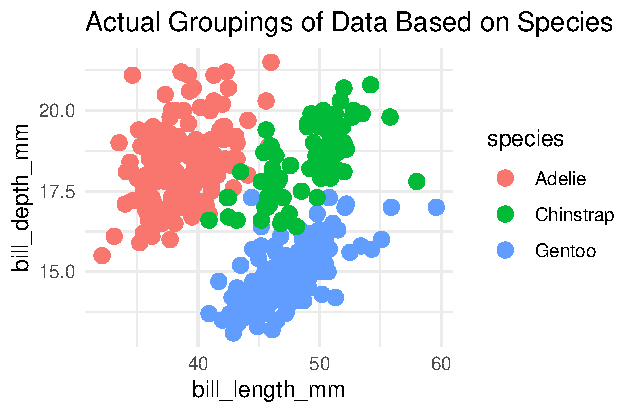
\includegraphics{K-Means-Mini-Demo_files/figure-pdf/unnamed-chunk-7-1.pdf}
\end{center}

\begin{itemize}
\tightlist
\item
  Visually, how well do you think \(K\)-means captured the underlying
  species structure of the data?
\end{itemize}

\textbf{Answer.} YOUR ANSWER HERE

\section{\texorpdfstring{Tuning \(K\)}{Tuning K}}\label{tuning-k}

\begin{itemize}
\item
  To implement K-means clustering we must choose an appropriate K! Use
  the following example to see the two different extreme situations.
  Typically, the ideal \(K\) is somewhere between the two extremes.
\item
  \textbf{Minimum:} \(K = 2\) groups/clusters
\item
  \textbf{Maximum:} \(K = n\) groups/clusters (one observation per
  cluster)
\end{itemize}

What happens in the \(K\)-means algorithm if \(K = n\)?

\textbf{Answer.} YOUR ANSWER HERE

Let's consider anywhere from \(K = 2\) to \(K = 20\) clusters.

\begin{Shaded}
\begin{Highlighting}[]
\FunctionTok{set.seed}\NormalTok{(}\DecValTok{244}\NormalTok{)}

\NormalTok{k\_2  }\OtherTok{\textless{}{-}} \FunctionTok{kmeans}\NormalTok{(}\FunctionTok{scale}\NormalTok{(penguins\_reduced), }\AttributeTok{centers =} \DecValTok{2}\NormalTok{)}
\NormalTok{k\_20 }\OtherTok{\textless{}{-}} \FunctionTok{kmeans}\NormalTok{(}\FunctionTok{scale}\NormalTok{(penguins\_reduced), }\AttributeTok{centers =} \DecValTok{20}\NormalTok{)}

\NormalTok{penguins\_reduced }\SpecialCharTok{\%\textgreater{}\%} 
  \FunctionTok{mutate}\NormalTok{(}\AttributeTok{cluster\_2 =} \FunctionTok{as.factor}\NormalTok{(k\_2}\SpecialCharTok{$}\NormalTok{cluster)) }\SpecialCharTok{\%\textgreater{}\%} 
  \FunctionTok{ggplot}\NormalTok{(}\FunctionTok{aes}\NormalTok{(}\AttributeTok{x =}\NormalTok{ bill\_length\_mm, }\AttributeTok{y =}\NormalTok{ bill\_depth\_mm, }\AttributeTok{color =}\NormalTok{ cluster\_2)) }\SpecialCharTok{+} 
    \FunctionTok{geom\_point}\NormalTok{(}\AttributeTok{size =} \DecValTok{3}\NormalTok{) }\SpecialCharTok{+} 
    \FunctionTok{labs}\NormalTok{(}\AttributeTok{title =} \StringTok{"K = 2"}\NormalTok{)}
\end{Highlighting}
\end{Shaded}

\begin{center}
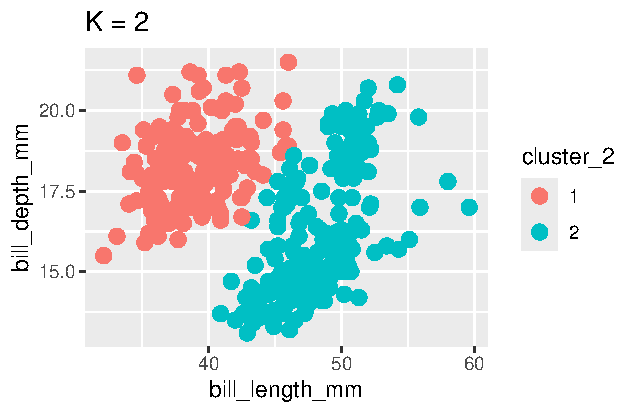
\includegraphics{K-Means-Mini-Demo_files/figure-pdf/unnamed-chunk-8-1.pdf}
\end{center}

\begin{Shaded}
\begin{Highlighting}[]
\NormalTok{penguins\_reduced }\SpecialCharTok{\%\textgreater{}\%} 
  \FunctionTok{mutate}\NormalTok{(}\AttributeTok{cluster\_20 =} \FunctionTok{as.factor}\NormalTok{(k\_20}\SpecialCharTok{$}\NormalTok{cluster)) }\SpecialCharTok{\%\textgreater{}\%} 
  \FunctionTok{ggplot}\NormalTok{(}\FunctionTok{aes}\NormalTok{(}\AttributeTok{x =}\NormalTok{ bill\_length\_mm, }\AttributeTok{y =}\NormalTok{ bill\_depth\_mm, }\AttributeTok{color =}\NormalTok{ cluster\_20)) }\SpecialCharTok{+} 
    \FunctionTok{geom\_point}\NormalTok{(}\AttributeTok{size =} \DecValTok{3}\NormalTok{) }\SpecialCharTok{+} 
    \FunctionTok{labs}\NormalTok{(}\AttributeTok{title =} \StringTok{"K = 20"}\NormalTok{) }\SpecialCharTok{+} 
    \FunctionTok{scale\_color\_manual}\NormalTok{(}\AttributeTok{values =} \FunctionTok{rainbow}\NormalTok{(}\DecValTok{20}\NormalTok{))}
\end{Highlighting}
\end{Shaded}

\begin{center}
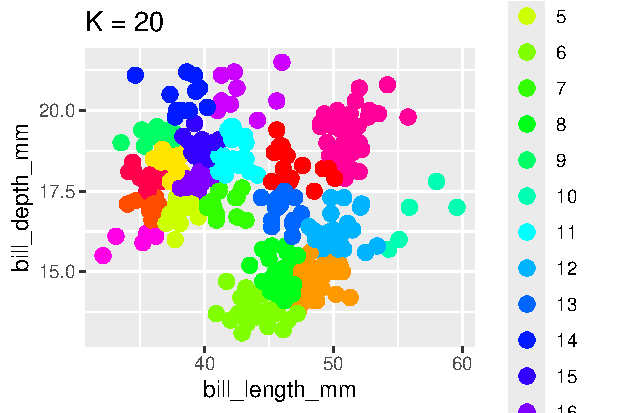
\includegraphics{K-Means-Mini-Demo_files/figure-pdf/unnamed-chunk-8-2.pdf}
\end{center}

What are your general impressions?

\textbf{Answer.} YOUR ANSWER HERE

\section{Finding Ideal K Value:
Silhoutte}\label{finding-ideal-k-value-silhoutte}

\begin{itemize}
\item
  The \emph{average silhouette approach} measures the quality of a
  clustering. That is, it determines how well each object lies within
  its cluster.

  \begin{itemize}
  \tightlist
  \item
    To do so, it maximizes the distance between clusters and minimizes
    distance within clusters.
  \end{itemize}
\item
  A high average silhouette indicates a good clustering.
\item
  Given a range of possible K values, the optimal number of clusters (K)
  is the one that maximizes the average silhouette.
\end{itemize}

We can use a built-in silhouette method in the \texttt{fviz\_nbclust}
function to compute the average silhouette for various K values.

\begin{Shaded}
\begin{Highlighting}[]
\FunctionTok{fviz\_nbclust}\NormalTok{(}\FunctionTok{scale}\NormalTok{(penguins\_reduced), kmeans, }\AttributeTok{method=}\StringTok{\textquotesingle{}silhouette\textquotesingle{}}\NormalTok{)}
\end{Highlighting}
\end{Shaded}

\begin{center}
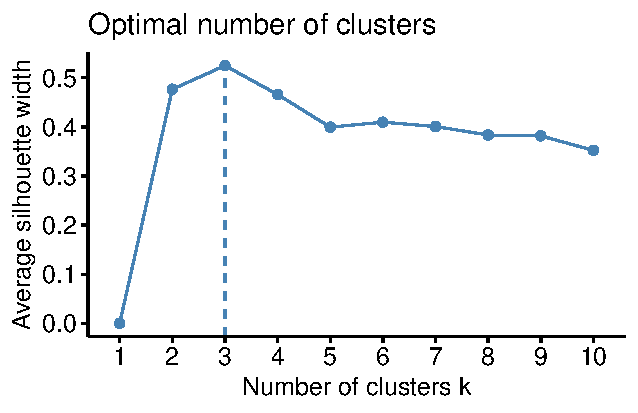
\includegraphics{K-Means-Mini-Demo_files/figure-pdf/unnamed-chunk-9-1.pdf}
\end{center}

Based on the \emph{average silhouette approach}, what is the optimal
\(K\) value?

\textbf{Answer.} YOUR ANSWER HERE

\section{Experimenting with Distance
Metrics}\label{experimenting-with-distance-metrics}

We can use the \texttt{Kmeans} method (notice the ``K'' is capitalized
in this function name) from the \texttt{amap} library to specify how we
are measuring distance in the K-means algorithm.

\begin{Shaded}
\begin{Highlighting}[]
\FunctionTok{set.seed}\NormalTok{(}\DecValTok{244}\NormalTok{)}
\NormalTok{k\_2\_manattan }\OtherTok{=} \FunctionTok{Kmeans}\NormalTok{(}\FunctionTok{scale}\NormalTok{(penguins\_reduced), }\AttributeTok{centers =} \DecValTok{3}\NormalTok{, }
                      \AttributeTok{method =} \StringTok{"manhattan"}\NormalTok{)}
\NormalTok{k\_2\_euclid }\OtherTok{=} \FunctionTok{Kmeans}\NormalTok{(}\FunctionTok{scale}\NormalTok{(penguins\_reduced), }\AttributeTok{centers =} \DecValTok{3}\NormalTok{, }
                    \AttributeTok{method =} \StringTok{"euclidean"}\NormalTok{)}
\NormalTok{k\_2\_maxnorm }\OtherTok{=} \FunctionTok{Kmeans}\NormalTok{(}\FunctionTok{scale}\NormalTok{(penguins\_reduced), }\AttributeTok{centers =} \DecValTok{3}\NormalTok{, }
                     \AttributeTok{method =} \StringTok{"maximum"}\NormalTok{)}



\FunctionTok{fviz\_cluster}\NormalTok{(k\_2\_euclid, }\AttributeTok{data =} \FunctionTok{scale}\NormalTok{(penguins\_reduced), }
             \AttributeTok{main =} \FunctionTok{sprintf}\NormalTok{(}\StringTok{"K = \%d Clusters w/ Manhattan Distance"}\NormalTok{, }\DecValTok{3}\NormalTok{))}
\end{Highlighting}
\end{Shaded}

\begin{center}
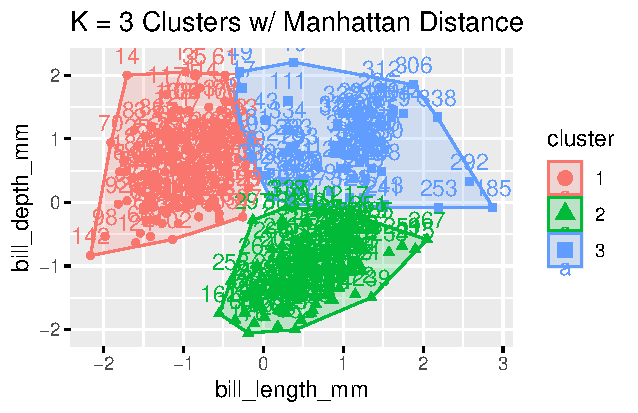
\includegraphics{K-Means-Mini-Demo_files/figure-pdf/unnamed-chunk-10-1.pdf}
\end{center}

\begin{Shaded}
\begin{Highlighting}[]
\FunctionTok{fviz\_cluster}\NormalTok{(k\_2\_manattan, }\AttributeTok{data =} \FunctionTok{scale}\NormalTok{(penguins\_reduced),}
             \AttributeTok{main =} \FunctionTok{sprintf}\NormalTok{(}\StringTok{"K = \%d Clusters w/ Manhattan Distance"}\NormalTok{, }\DecValTok{3}\NormalTok{))}
\end{Highlighting}
\end{Shaded}

\begin{center}
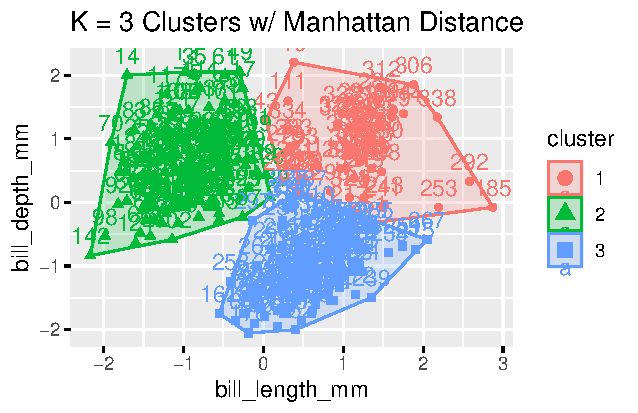
\includegraphics{K-Means-Mini-Demo_files/figure-pdf/unnamed-chunk-10-2.pdf}
\end{center}

\begin{Shaded}
\begin{Highlighting}[]
\FunctionTok{fviz\_cluster}\NormalTok{(k\_2\_maxnorm, }\AttributeTok{data =} \FunctionTok{scale}\NormalTok{(penguins\_reduced),}
             \AttributeTok{main =} \FunctionTok{sprintf}\NormalTok{(}\StringTok{"K = \%d Clusters w/ Manhattan Distance"}\NormalTok{, }\DecValTok{3}\NormalTok{))}
\end{Highlighting}
\end{Shaded}

\begin{center}
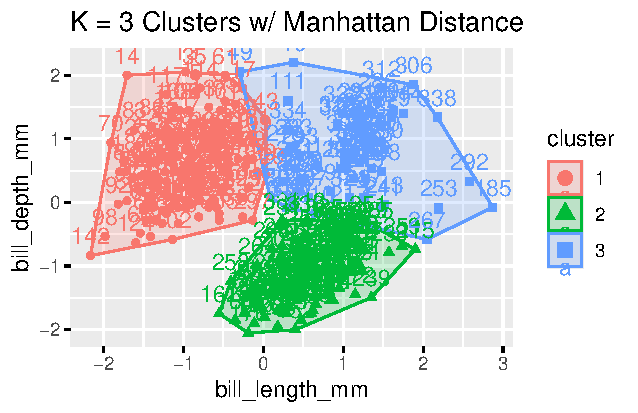
\includegraphics{K-Means-Mini-Demo_files/figure-pdf/unnamed-chunk-10-3.pdf}
\end{center}

Try changing \(K\) to equal 3\$ in the code chunk above. How do the
clusterings using the 3 distance metrics compare? What do you generally
observe?

\textbf{Answer.} YOUR ANSWER HERE

Modify the code in the chunk above so that we can easily change the
value of K (rather than making sure to change K manually in every line).
In general coding practices, is called \emph{extracting out a constant.}




\end{document}
